
\begin{figure}
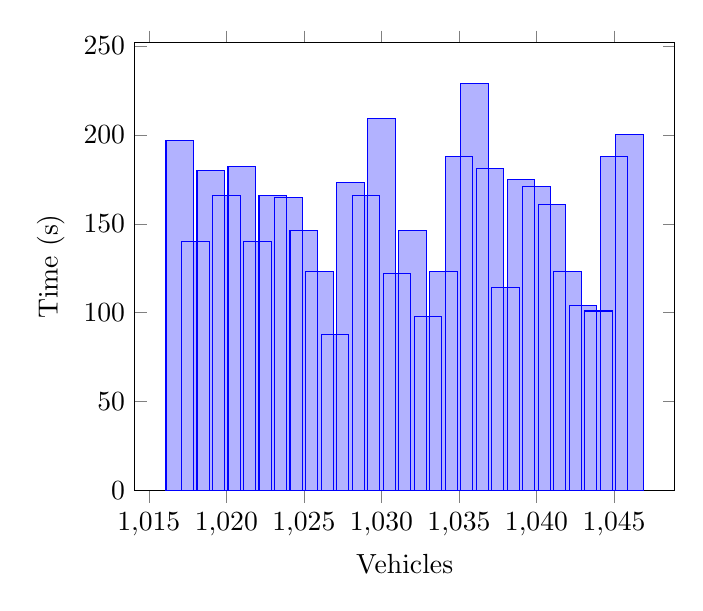
\begin{tikzpicture}
\begin{axis}[
legend style={anchor=west},
xlabel=Vehicles,
ylabel=Time (s),
ymin=0,
ybar,
]
\addplot coordinates {
(1017, 197)
(1025, 146)
(1028, 173)
(1043, 104)
(1032, 146)
(1042, 123)
(1041, 161)
(1040, 171)
(1046, 200)
(1045, 188)
(1044, 101)
(1037, 181)
(1018, 140)
(1019, 180)
(1023, 166)
(1022, 140)
(1029, 166)
(1038, 114)
(1033, 98)
(1031, 122)
(1035, 188)
(1039, 175)
(1036, 229)
(1030, 209)
(1024, 165)
(1027, 88)
(1026, 123)
(1021, 182)
(1020, 166)
(1034, 123)
};

\end{axis}
\end{tikzpicture}
\label{tik:time:0:97}
\caption{0 percent diving with GSC on route $97$}
\end{figure}
